\documentclass[addpoints,12pt]{exam}
\newcommand{\ds}{\displaystyle}
\usepackage[margin=0.8in]{geometry}
\usepackage{subcaption}
\usepackage{tikz}
\usepackage{amssymb,amsmath,graphicx,wrapfig,verbatim,wasysym, enumitem,psfragx,color}
\usepackage{multicol}

\usepackage{xpatch}

\makeatletter
\xpatchcmd{\@fillin@relay}
  {\hbox to #1{\hrulefill}\fi}
  {\hbox{\framebox[#1]{\rule{0pt}{2ex}}}\fi}
  {}{}
\makeatother

%\usepackage{fancyhdr}
%\setlength{\headheight}{13.6pt}
%\pagestyle{fancy}
%\lhead{Math 222}
%\chead{ Midterm 1 }

%\rhead{Spring 2022}

\def\FillInBlank{\rule{3truein} {.01truein}}


% Choose one option (bubbles)
\newcommand{\chooseone}{{\Large$\Circle$\ \ }}


\newcommand{\myleft}{\makebox[.4\textwidth]{First Name:\enspace\hrulefill}}
\newcommand{\myright}{\makebox[.4\textwidth]{Last Name:\enspace\hrulefill}}
\header{\oddeven{\myleft}{}}
    {}
    {\oddeven{\myright}{}}

\footrule

\footer{Math 211}
     {Midterm 1 Practice Exam}
     {Page \thepage\ of \numpages}

\begin{document}

\begin{questions}


\question Clearly mark the correct answer for each of the following by completely filling in the
appropriate bubble. \textbf{No justification is needed.}


\begin{parts}

\part[2] \textbf{(Multiple Choice)} The cost of producing $x$ ounces of gold from a new gold
mine is $C(x)$ dollars. What does the statement $C'(500) = 17$ mean?




\begin{itemize}[label={}]
\item \chooseone The total cost to produce 17 ounces of gold is approximately \$500.

\item \chooseone After 500 ounces of gold have been produced, the average production cost is
\$17/ounce. So the cost of producing 500 ounces is about \$17/ounce.

\item \chooseone After 500 ounces of gold have been produced, the rate at which the
production cost is increasing is \$17/ounce. So the cost of producing the 500th (or 501st) ounce
is about \$17.
\item \chooseone After 17 ounces of gold have been produced, the average production cost is
\$500/ounce. So the cost of producing 17 ounces is about \$500/ounce.
\end{itemize}

\medskip




\part[2] \textbf{(True/False)} If $f(t)$ is the function describing (in feet) the water level in a lake at
time $t$ (where $t$ is in hours), and $f'(3)=10$ and $f''(3)=-2$, then the water level is rising at
$t=3$, but the rate is slowing.

\begin{itemize}[label={}]
\item \chooseone True
\item \chooseone False
\end{itemize}

\vfill




\part[2] \textbf{(True/False)} The graph below describes a function in $x$.
\begin{itemize}[label={}]
\item \chooseone True
\item \chooseone False
\end{itemize}
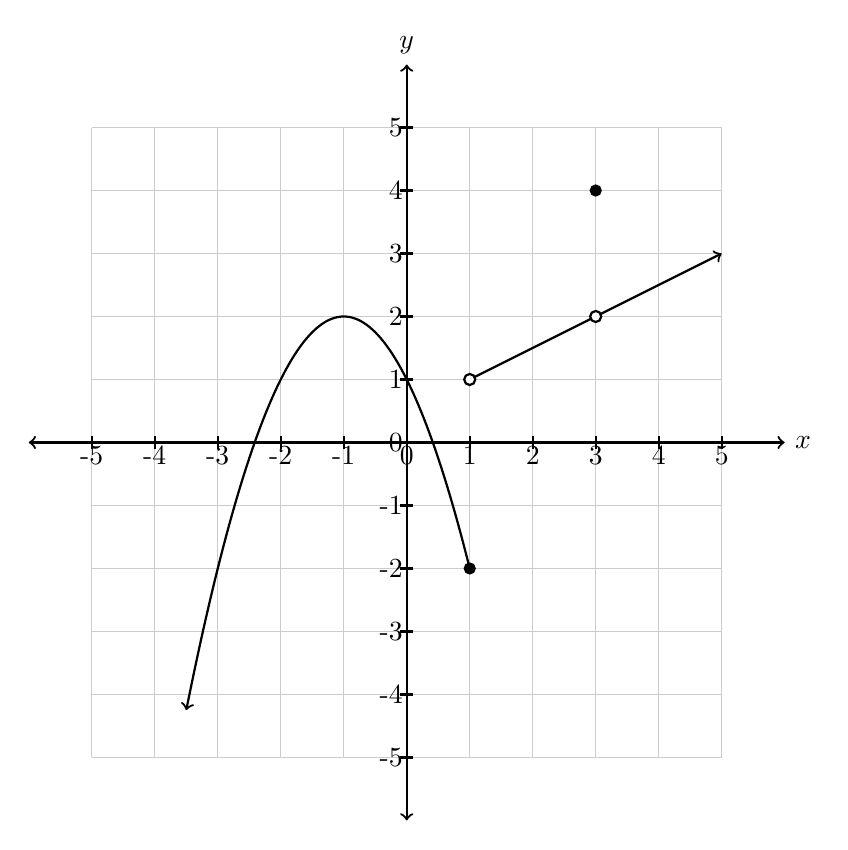
\begin{tikzpicture}[scale=.8]
\draw[gray!40] (-5, -5) grid[step=1] (5, 5);
\draw[<->,thick,black] (-6,0)--(6,0) node[right]{$x$};
\draw[<->, thick,black] (0,-6)--(0,6) node[above]{$y$};
\foreach \x in {-5,-4,...,5}
\draw[thick] (\x,-.1) --(\x,.1) node[below]{\x};
\foreach \y in {-5,-4,...,5}
\draw[thick] (-.1,\y) --(.1,\y) node[left] {\y};
\draw[domain=-3.5:1,samples=100, thick,<-] plot ({\x},{-(\x+1)^2+2});
\draw[domain=1:5,samples=100,thick,->] plot ({\x},{(\x/2+0.5});
\draw[fill=black] (3,4) circle[radius=0.25em];
\draw[fill=black] (1,-2) circle[radius=0.25em];

\draw[fill=white,thick] (3,2) circle[radius=0.25em];
\draw[fill=white,thick] (1,1) circle[radius=0.25em];
\end{tikzpicture}




\vfill

\end{parts}

\newpage


\newpage


\question Calculate the derivative of each function. You do not need to simplify your answer.

\begin{parts}




\part[5] $g(x)=\dfrac{4}{x^3} + 7$
\vspace{2in}

\part[5] $F(x)=(x+1)(2x+3)$

\vspace{2in}

\part[5] $r(x)=\ds\sqrt{2x-3}$

\vspace{2in}

\part[5] $f(x)=(x^2+2x)^8$

\vspace{2in}




\end{parts}

\newpage


\question Find each limit. Show all work. Simplify your final answers.

\begin{parts}

\part[4] $\ds \lim_{x\to 3} \dfrac{ x^2-x-6}{x^2+2x-15}$

\vfill


\part[4] $\displaystyle \lim_{x\to 0}\dfrac{3x-5}{x^2+3}$

\vfill

\end{parts}

\newpage

\question[11] Find an equation for the tangent line of $f(x)=x^3-5x^2+2$ at $x=1$. Show all
work.

\newpage

\question[8] Find $f''(x)$ of $f(x)=4x(x+1)$. You do not need to simplify your final answer. Show
all work.


\newpage




\question A baseball bat manufacturer finds that the cost of making $x$ bats is $C(x)=40+10x$,
and the revenue in selling $x$ bats is $R(x)=28x-2x^2$.

\begin{parts}
\part[5] Find all $x$ value(s) where $R(x)=C(x)$. Show your work.

\vspace{2in}

\part[3] Find the \textbf{marginal revenue function} $MR(x)$ and evaluate $MR(2)$. You do not
need to simplify your final numerical answer.

\vspace{2in}

\part[2] Find the \textbf{average cost function} $AC(x)$.

\vspace{1in}




\part[4] Find the \textbf{marginal average cost function} $MAC(x)$ and evaluate $MAC(2)$. You
do not need to simplify your final numerical answer.

\vfill

\vfill




\end{parts}

\newpage


\question Consider the function $y=f(x)$ below. Answer the following questions.
​
​        \begin{tikzpicture}[scale=.99]
​        ​        \draw[gray!60] (-5, -5) grid[step=1] (5, 5);
​        ​        \draw[<->,thick,black] (-5,0)--(5,0) node[right]{$x$};
​        ​        \draw[<->, thick,black] (0,-5)--(0,5) node[above]{$y$};
​        ​        \foreach \x in {-5,-4,...,5}
​        ​        \draw[thick] (\x,-.1) --(\x,.1) node[below] {\small \x};
​        ​        \foreach \y in {-5,-4,...,5}
​        ​        \draw[thick] (-.1,\y) --(.1,\y) node[left] {\small \y};
​        ​        \draw[domain=-3.5:4.25,samples=200,thick,<->] plot
({\x},{(3*\x*\x*\x*\x-8*\x*\x*\x-30*\x*\x+72*\x)/50});
​        ​        \node at (4,2.7) {$y=f(x)$};
​        \end{tikzpicture}


\begin{parts}
\part[2] For which $x$-value(s) is $f'(x)=0$? Briefly (one sentence) explain your answer.

\vspace{1in}

\part[2] Is $f'(-1)$ positive, negative, or zero? Briefly (one sentence) explain your answer.

\vspace{1in}


\part[2] Is $f'(2)$ positive, negative, or zero? Briefly (one sentence) explain your answer.

\vspace{1in}

\end{parts}




\newpage

\question[10] Use the (limit) definition of the derivative,
$$\displaystyle f'(x)=\lim_{h\to 0}\frac{f(x+h)-f(x)}{h},$$ to compute $f'(x)$ for $f(x)=3x^2-4$.

\newpage


\question For the graph of $y=f(x)$ below:

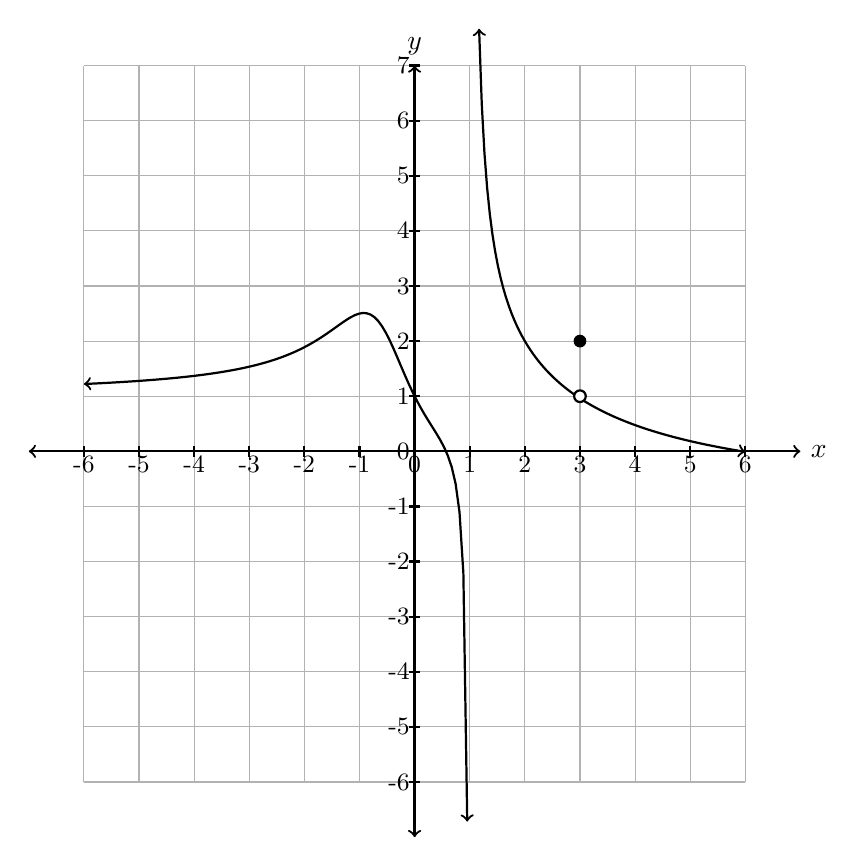
\begin{tikzpicture}[scale=.7]
\draw[gray!60] (-6, -6) grid[step=1] (6, 7);
\draw[<->,thick,black] (-7,0)--(7,0) node[right]{$x$};
\draw[<->, thick,black] (0,-7)--(0,7) node[above]{$y$};
\foreach \x in {-6,-5,...,6}
\draw[thick] (\x,-.1) --(\x,.1) node[below] {\small \x};
\foreach \y in {-6,-5,...,7}
\draw[thick] (-.1,\y) --(.1,\y) node[left] {\small \y};
 \draw[domain=-6:0.955,samples=100, thick,<->] plot ({\x},{-(\x*\x-2*\x)/(\x*\x*\x-1)+1});
 \draw[domain=1.17:6,samples=100,thick,<->] plot ({\x},{-3*(\x*\x-2*\x)*\x/(\x*\x*\x-1)+2});
\draw[fill=white,thick] (3,1) circle[radius=0.3em];
\draw[fill=black] (3,2) circle[radius=0.3em];
\end{tikzpicture}


\begin{parts}

\part[2] Give all $x$-values where $f(x)$ is discontinuous.

\vspace{1in}

\part[4] Find each value, if possible. If not possible, write DNE.
\vspace{0.5in}

(a) $\displaystyle \lim_{x\to 1^-} f(x)=$

\vspace{0.5in}

(b) $\displaystyle \lim_{x\to 1^+} f(x)=$
\vspace{0.5in}


(c) $\displaystyle \lim_{x\to 1} f(x)=$
\vspace{0.5in}

(d) $\displaystyle \lim_{x\to 3} f(x)=$
\vspace{0.5in}




\end{parts}

\newpage


\question
\begin{parts}

\part[4] Given the graph of $y=f(x)$ below, give the domain and the range of $f(x)$. Use interval
notation.

\begin{minipage}{0.4\textwidth}


Domain:

 \vspace{1in}

 Range:

 \vspace{2in}

\end{minipage}
\begin{minipage}{0.4\textwidth}
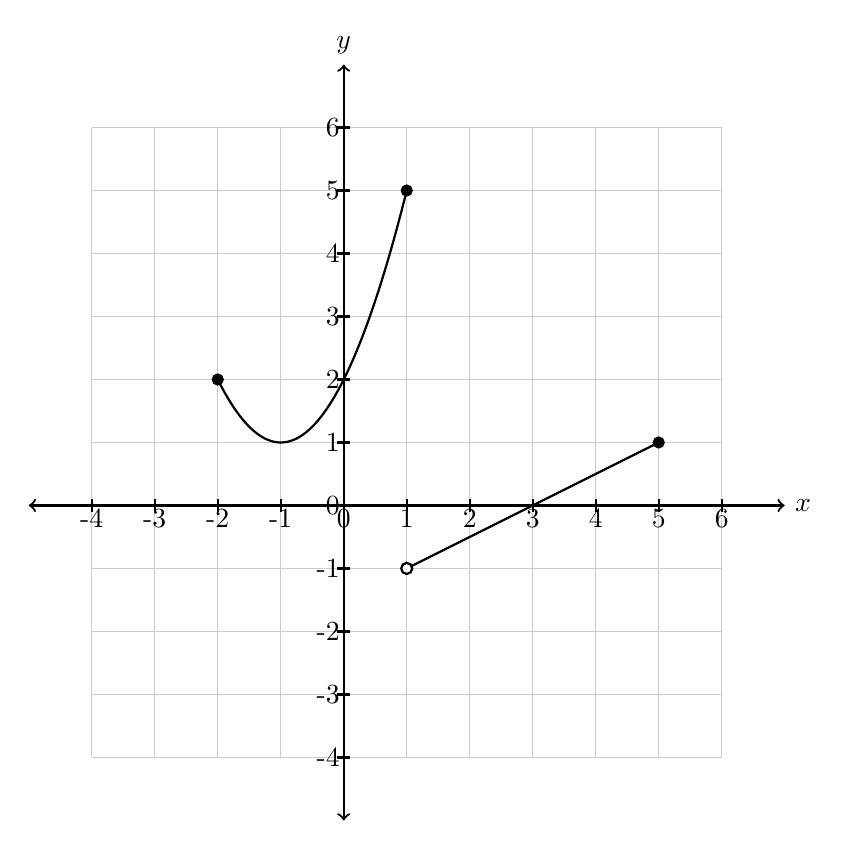
\begin{tikzpicture}[scale=.8]
\draw[gray!40] (-4, -4) grid[step=1] (6, 6);
\draw[<->,thick,black] (-5,0)--(7,0) node[right]{$x$};
\draw[<->, thick,black] (0,-5)--(0,7) node[above]{$y$};
\foreach \x in {-4,-3,...,6}
\draw[thick] (\x,-.1) --(\x,.1) node[below]{\x};
\foreach \y in {-4,-3,...,6}
\draw[thick] (-.1,\y) --(.1,\y) node[left] {\y};
\draw[domain=-2:1,samples=100, thick,-] plot ({\x},{(\x+1)^2+1});
\draw[domain=1:5,samples=100,thick,-] plot ({\x},{\x/2-1.5});
\draw[fill=black] (-2,2) circle[radius=0.25em];
\draw[fill=black] (1,5) circle[radius=0.25em];
\draw[fill=black] (5,1) circle[radius=0.25em];
\draw[fill=white,thick] (1,-1) circle[radius=0.25em];
\end{tikzpicture}
\end{minipage}

\part[4] Simplify $\dfrac{x^2}{4\sqrt{x}}$ to the form $ax^b$, where $a$ and $b$ are both
numbers.
\vspace{1.5in}

\part[3] For $f(x)=2x-1$ and $g(x)=\sqrt{x+3}$, Write down expressions for each function
composition. You do not need to simplify.

\vspace{0.5in}

$f(g(x))=$

\vspace{0.5in}

$g(f(x))=$


\vspace{0.5in}

$f(f(x))=$

\end{parts}




\end{questions}

\end{document}
